\documentclass[sigplan,screen]{acmart}


%% Contributed by Gregor von Laszewski
\usepackage{textcomp}
\usepackage{hyperref}
%\usepackage[table]{xcolor}

\usepackage{todonotes}
\newcommand{\TODO}[1]{\todo[inline]{#1}}
\newcommand{\NOTE}[1]{\textcolor{red}{[NOTE: #1]}}
\newcommand{\FILE}[1]{\todo[inline,color=green!20]{File: #1}}

\newcommand{\GITHUB}[1]{\todo[inline,color=green!20]{
\href{https://github.com/laszewsk/mlcommons-uva/issues/#1}{GitHub Issue #1}}}


\setcopyright{none}
\settopmatter{printacmref=false}
\renewcommand\footnotetextcopyrightpermission[1]{}

%\usepackage{minted}
%\setminted{fontsize=\footnotesize,xleftmargin=1.5\parindent}

\usepackage{fancyvrb}

% \usepackage{color}
% \usepackage{listings}
%\usepackage{xcolor}
%\usemintedstyle{trac}
%\definecolor{mblue}{rgb}{0.27,0.33,0.53}

\definecolor{friendlybg}{HTML}{f0f0f0}
\definecolor{lightgray}{rgb}{.9,.9,.9}
\definecolor{darkgray}{rgb}{.4,.4,.4}
\definecolor{purple}{rgb}{0.65, 0.12, 0.82}

% \lstdefinelanguage{bash}{
%   keywords={cms, cd},
%   keywordstyle=\color{blue}\bfseries,
%   keywords=[2]{set},
%   keywordstyle=[2]\color{green}\bfseries,
%   identifierstyle=\color{black},
%   sensitive=false,
%   comment=[l]{//},
%   morecomment=[s]{/*}{*/},
%   commentstyle=\color{purple}\ttfamily,
%   stringstyle=\color{red}\ttfamily,
%   morestring=[b]',
%   morestring=[b]"
% }

% \lstset{
%   language=bash,
%   extendedchars=true,
%   basicstyle=\footnotesize\ttfamily,
%   showstringspaces=false,
%   showspaces=false,
%   tabsize=2,
%   breaklines=true,
%   showtabs=false
% }

%\setcopyright{acmcopyright}
%\copyrightyear{2018}
%\acmYear{2018}
%\acmDOI{XXXXXXX.XXXXXXX}

%\acmConference[Conference acronym 'XX]{Make sure to enter the correct
%  conference title from your rights confirmation emai}{June 03--05,
%  2018}{Woodstock, NY}

%\acmBooktitle{Woodstock '18: ACM Symposium on Neural Gaze Detection,
%  June 03--05, 2018, Woodstock, NY} 
%\acmPrice{15.00}
%\acmISBN{978-1-4503-XXXX-X/18/06}

%%\acmSubmissionID{123-A56-BU3}

%%\citestyle{acmauthoryear}

\begin{document}

\newcommand{\TITLE}{Improving the MLCommons CloudMask Benchmark}

\title{\TITLE}

\author{Gregor von Laszewski}
\email{laszewski@gmail.com}
\orcid{0000-0001-9558-179X}
\authornote{Corresponding author}
\affiliation{%
  \institution{University of Virginia}
  \streetaddress{Biocomplexity Institute and Initiative\\
Town Center Four\\
994 Research Park Boulevard}
  \city{Charlottesville}
  \state{VA}
  \postcode{22911}
  \country{USA}
}

\author{Varshita Chennamsetti,\\ 
Laiba Mehnaz,\\
Ruochen Gu, \\
Sergey Samsonau}
\affiliation{%
  \institution{New York University}
  \streetaddress{Center for Data Science\\
60 5th Ave}
  \city{New York}
  \state{NY}
  \postcode{10011}
  \country{USA}
}

\author{Juri Papaya, \\Samuel Jackson}
\email{juri.papay@stfc.ac.uk}
\affiliation{%
  \institution{Rutherford Appleton Laboratory}
  \streetaddress{Harwell Campus}
  \city{Didcot}
  \postcode{OX11 0QX}
  \country{UK}
}

\author{Geoffrey C. Fox}
\email{gcfexchange@gmail.com}
\affiliation{%
  \institution{University of Virginia}
  \streetaddress{Biocomplexity Institute\\
Town Center Four\\
994 Research Park Boulevard}
  \city{Charlottesville}
  \state{VA}
  \postcode{22911}
  \country{USA}
}

%%
%% By default, the full list of authors will be used in the page
%% headers. Often, this list is too long, and will overlap
%% other information printed in the page headers. This command allows
%% the author to define a more concise list
%% of authors' names for this purpose.
\renewcommand{\shortauthors}{von Laszewski et al.}

%%
%% The abstract is a short summary of the work to be presented in the
%% article.
\begin{abstract}

This paper describes efforts to improve the MLCommons Science benchmark. This focuses on several important activities. It includes the replacement of numerical accuracy that is now based on a continuous evaluation function replacing the previous Boolean value-based evaluation function as previously any run beyond epoch one returned the same value. The new evaluation function enables more precise and granular assessment of accuracy throughout the benchmark execution. We also improved the handling of hyper-parameter varied benchmarks to analyze their effect while varying them and recording their impact on the accuracy. The benchmarks are ported and executed on various HPC machines and to increase usability and portability to other machines the user manual has been significantly updated while showcasing specific adaptations for different HPC resources. Lastly, we created a leaderboard with the best parameters that we found and intend to submit to MLCommons. These enhancements demonstrate an increase in the a community-driven approach to benchmarking as part of the MLCommons Science working group. 

\end{abstract}

%%
%% The code below is generated by the tool at http://dl.acm.org/ccs.cfm.
%% Please copy and paste the code instead of the example below.
%%
\begin{CCSXML}
<ccs2012>
   <concept>
       <concept_id>10010147.10010257.10010321</concept_id>
       <concept_desc>Computing methodologies~Machine learning algorithms</concept_desc>
       <concept_significance>500</concept_significance>
       </concept>
   <concept>
       <concept_id>10002944.10011123.10011124</concept_id>
       <concept_desc>General and reference~Metrics</concept_desc>
       <concept_significance>500</concept_significance>
       </concept>
 </ccs2012>
\end{CCSXML}

\ccsdesc[500]{Computing methodologies~Machine learning algorithms}
\ccsdesc[500]{General and reference~Metrics}


%%
%% Keywords. The author(s) should pick words that accurately describe
%% the work being presented. Separate the keywords with commas.
\keywords{MLCommons, science benchmark, cloud masking, cloudmesh}


\received{June 2023}
%\received[revised]{12 March 2009}
%\received[accepted]{5 June 2009}

{\huge\bf \TITLE}


\tableofcontents

\listoffigures
\listoftables

\listoftodos{List of todos}

\section{Open-questions}

\TODO{Gregor put his thought about this in this paper including a function. \\ 

1. Is the data randomly inputted to the model? answer in paper

2. Is the random number generating different random numbers with different runs? TBD. but with 1 we generate different numbers

3. Is the random seed set properly? See the function I propose}

\TODO{4. The run 3 produces good values, can we replicate the visualization of that 
with smaller epoch runs? 

5. The analysis script is not committed.
}

\TODO{6. (no time to address) Does the utilization of the floating point numbers create numerical instabilities? Eg: Catastrophic cancellation}

\TODO{7. (not time to address) Does it make a difference to have a 64-bit or 32-bit? 6.1. What are we using in bits?}

\TODO{7. check all abbreviations and introduce if missing at first use}

\clearpage

\maketitle

\section{Introduction}


With artificial intelligence (AI), machine learning (ML) and deep learning (DL) becoming a powerful technologies transforming many aspects of the scientific analysis of data, several scientific fields are yet to fully benefit from advances in AI. Despite the rising excitement around AI, the scientific community has yet to systematically integrate AI methods and tools into the research process. In particular, more understanding is required on the applicability of AI/ML/DL to various scientific problems, and the role of large scale computing resourceso, datasets, explainability and robustness of AI/ML/DL techniques, the role of small-scale devices on AI/ML, AI/ML-specific algorithms, and scalability of AI/ML techniques with varying volumes of data or varying computational capabilities \cite{mlcommons-benchmark-2023}. 

Hence, there is a need for an initiative to increase awareness and push forward innovation in scientific fields where the potential for AI is huge but underexplored. To increase better understanding of the impact of AI and deep learning (DL) 
MLCommons\textsuperscript{\texttrademark} \cite{www-mlcommons} tries to understand the impact of AI and DL   
on the utilization of needed resources, but also on exemplars where DL works or has issues.

MLCommons is a community effort by leading government agencies, universities, and commercial companies to promote scientific AI benchmarks. Within MLcommons the science working group \cite{Thiyagalingam2022AIBF} is a research group, that has so far developed four scientific benchmarks in varying fields such as atmospheric sciences, solid-state physics, healthcare, and earthquake forecasting \cite{las23-insights-mlcommons-education} focusing on furthering the accuracy of these applications by developing new and improving existing algorithms. 

% \subsection{Cloudmasking}

In this paper, efforts are presented to improve the MLCommos science benchmark for cloudmask \cite{Thiyagalingam2022AIBF}. Cloudmask is an application to identify the cloud coverage within many different images. The presence of clouds is an obstacle to using clear images of the earth's surface. Hence it is advantageous to be able to identify pixels in images that are covered by clouds. On the other hand, cloud coverage itself could also be a topic of interest so it is usable in applications that look at cloud coverage instead trying to use it to remove clouds to create clear earth surface images. 
To facilitate such an advanced application the objective of the MLCommons Science cloudmask benchmark is to identify cloud pixels given a satellite image through segmentation. 

Throughout the paper, the term {\em cloudmasking} is used for the process of identifying clouds, while the resulting data structure identifying which pixel is covered by a cloud over the observation area is called a {\em cloudmask}.

\TODO{review the next section once paper is ok and fix accordingly}

The paper is structured as follows. First, we give an introduction to the MLCommons Science Benchmark group goals and summarize the difference to regular benchmarks that may only be concerned with time and space (Section ~\ref{sec:mlcommons}). Next, we introduce some background work focusing on cloudmasking (Section \ref{sec:related}. We then introduce our benchmark methodology (Section \ref{sec:bench-method}. This includes the description of the data used for the benchmark, the model used for the discovery of the cloudmask and the modification to the accuracy value, modifications that have been conducted to enhance and simplify logging focusing on human readable and easy machine parsable benchmark logs that comply with submissions to MLcommons. The next section focuses on the execution of the benchmark experiments discussing in detail which experiments and compute resources have been used. It also includes a detailed analysis of the benchmarks while varying some hyper-parameters such as the number of epochs used. We finish this section with a leaderboard table that is being submitted to MLCommons while focusing on the best result identified by the various runs we conducted. We conclude the paper by summarizing our findings (Section \ref{sec:conclusion}). 


\section{MLCommons Science Benchmarking}
\label{sec:mlcommons}


One of the working groups in MLCommons is the Science Working Group \cite{Thiyagalingam2022AIBF}. The Science Working Group maintains four different benchmarks. It provides the data for training and testing purposes and defines a metric that needs to be reported by the user. 

While other MLCommons benchmarks and working groups focus on the benchmarking of resources and their impact on training and inference, the science working group's goals are to identify algorithms and applications that can solve a particular scientific application most accurately. This is accomplished by identifying appropriate hyperparameters that control the algorithm. In addition, it may also include modified data that enhance the data analysis. Although resource 
utilization is not the main focus it needs to be considered as resource limitations need to be understood where they provide a limiting factor. This includes runtime resource limitations of the capabilities of the GPU, the number of GPUs used, as well as the limitations of the IO system. Applications may differ significantly in terms of both their volume and type of data as well as the computational needs to conduct the data analysis. This may require heavy utilization of large-scale computing resources \cite{Farrell2021MLPerfHA}. However, it may also be including applications that can be run on the desktop while many repeated runs and configurations are explored \cite{las23-insights-mlcommons-education}. 

Hence, Scientific benchmarking is different from standard AI/ML benchmarking in that it focuses first on finding the best combination of algorithms and data resulting in the best accuracy of the scientific result. Second, it identifies needed hardware resources to document reproducibility and resource needs needed for today's scientific problems that have many parameters and potentially require a significant amount of computing and data resources. 


\section{Overview of Cloudmasking}

The European Space Agency (ESA) has deployed a series of satellites for monitoring of the global environment. Amongst these satellites, Sentinel-3 is focusing on ocean surface topography, sea surface temperature (SST), and land surface temperature (LST) \cite{www-sentinal-3}. The process of the retrieval of SST and SLT usually begins with cloud screening or masking, followed by the actual temperature estimation of the pixels that do not contain clouds. Cloud masking needs to be performed since the presence of clouds can distort the accurate estimations of temperature, making it a crucial step in the process of SST and LST estimation.

\subsection{Related Work in Cloudmasking}
\label{sec:related}

Several methods have been used for this task ranging from rule-based focused cloudmasking to deep learning based cloudmasking \cite{WIELAND2019111203,Yan2018CloudAC}.  Some of the rule based techniques include thresholding \cite{Saunders1986AnAS,Saunders1988AnIM} and Bayesian masking \cite{Merchant2005ProbabilisticPB}. 

{\bf Thresholding} consist of several threshold tests where spectral and spatial properties/signals of the images are compared with those ranges that are believed to be indicative of a {\em clear-sky} pixel. Other pixels that are not labeled as {\em clear-sky} are flagged as {\em cloudy} pixel. Thresholding was widely used from late 1980s to early 2000s. However since then a shift occurred that gradually transitioned away from threshold tests due to its limitations. First, threshold setting relies on domain expertise about indicators of cloudiness that may not be objective, which also makes later modification and updates difficult. Second, thresholds provide users no flexibility in the trade-off between SST coverage and SST bias. Thirdhird, threshold tests do not make use of all available prior information. These shortcomings of thresholding methods are improved by later developed Bayesian methods  \cite{unkown}.

\TODO{the refence to this is missing}

Bayesian methods were developed and started getting traction in the early 2000s. These methods deduce the probability of a clear sky over each pixel by applying Bayes' theorem. As a result, these Bayesian approaches are fully probabilistic and deduce pixels based on prior information and observations in images. Compared to threshold tests, Bayesian methods achieve better accuracy in predicting pixels' cloudiness, offer generality and conceptual clarity in their approach, and enhance maintainability and adaptability largely. 

{\bf Bayesian masks} use the Bayes theorem to provide probabilities based on the data provided of having a clear sky or not, per pixel. Using these probabilities and applying them to a given image, a cloud mask can be generated. Recently,  deep learning methods \cite{WIELAND2019111203,Yan2018CloudAC} have been applied that use computer vision models and treat the task of cloudmasking as an image segmentation model to generate the masks to identify the pixels that have clouds. A widely used model is the U-net model \cite{Ronneberger2015UNetCN} which is pre-trained and designed  using image segmentation while using large images.

More recently, the rise of deep learning has been applied to a new approach to cloud masking \cite{Thiyagalingam2022AIBF}. 


A small summary of accuracy results using different data and algorithms is shown in Table \ref{tab:datasets}. Throughout this paper we will comment on our contribution to this table and contrast how it compares as part of our documented results.

\TODO{sentinel 3 not listed in the table from previous work prior to us.}

\begin{table*}[!ht]
    \centering
    \caption{Related work, performance represents the accuracy per pixel for the cloud mask generated.}
    \label{tab:datasets}
    \resizebox{0.7\textwidth}{!}{
    \begin{tabular}{|l|c|l|l|l|l|}
    \hline
        {\bf} & {\bf Reference} & {\bf Dataset} & {\bf Ground-truth} & {\bf Model}  & {\bf Accuracy} \\ \hline
        1 & \cite{Merchant2005ProbabilisticPB} & ATSR-2 & Human annotation & Bayesian screening & 0.917\\ \hline
        2 & \cite{WIELAND2019111203} & Sentinal-2 & Software generated (QGIS) & U-Net & 0.90 \\ \hline
        3 & \cite{WIELAND2019111203} & Landsat TM & Software generated (QGIS) & U-Net & 0.89 \\ \hline
        4 & \cite{WIELAND2019111203} & Landsat ETM+ & Software generated (QGIS) & U-Net & 0.89 \\ \hline
        5 & \cite{WIELAND2019111203} & Landsat OLI & Software generated (QGIS) & U-Net & 0.91 \\ \hline
        6 & \cite{8401847} & GaoFen-1 & Human annotation & MFFSNet & 0.98, mIOU = 0.87 \\ \hline
        7 & \cite{unkown} & Sentinal-3 & ??  & ?? & ??? ?? \\ 
        \hline
    \end{tabular}
    }
\end{table*}

\section{MLCommons and MLCommons Science Working Group Benchmark Methodology}

As previously mentioned MLCommons has developed a number of AI-related benchmarks using GPUs to identify the efficiency of a variety of computing resources on a defined set of AI applications. This includes the impact on training and inference. MLCommons targets a wide set of resources from {\em tiny} to large-scale HPC computers. neIn fact, several of the largest academic computing centers have reported their results to MLCommons on these benchmarks. In \cite{las23-insights-mlcommons-education} we have provided a simple overview of some of these benchmarks and how they can be aligned with educational efforts.

The use of such AI benchmarks allows one to assess the relative performance of the benchmarks on resources in regard to them.
It also serves as a measurement to provide a guide on the effectiveness of a model and serves as a guide to improve the algorithm. 

But as stated in \cite{arxiv-mlperf} unlike other computation tasks, AI/ML algorithms and models are particularly difficult to benchmark, due to three unique challenges that are absent from other domains: optimizations that improve training throughput can increase the time to solution, training is stochastic and time to solution exhibits high variance, and software and hardware systems are so diverse that fair benchmarking with the same binary, code, and even hyperparameters is difficult. 

However, it is not sufficient to just look for existing benchmarks and measure their performance. In science, we are looking at finding the best scientific accurate value within available resources. 
Thus the science working group sets as its goal to identify methods on how to obtain the most accurate scientific results.
As earlier stated this can introduce a variety of factors that need to be identified and analysed. It includes but is not limited to 

\begin{itemize}
    \item algorithms
    \item hyperparameters
    \item effective training and validation workflows
    \item impact of data selection, augmentation, and injection
    \item impact of available resources
\end{itemize}

The MLCommons Science working group is looking at these and other related issues
\cite{mlcommons-benchmark-2023}.



\section{Benchmark Details for the Cloudmask Application}
\label{sec:bench-method}

This section includes details for the MLCommons Science Working group cloudmask application benchmark that is described in this paper. We address features related to the dataset, the model and changes to the existing accuracy value for better DL-based benchmarking, and logging. 

\subsection{Dataset}

As part of the cloud masking benchmark, we are provided with the satellite images from Sentinel-3 \cite{www-sentinal-3} for the task of cloud masking using deep learning. 
The dataset consists of a total of 1070 images, both captured at day and night. The dataset is split into train and test with 90\% used for training, and 10\% used for testing. 
Hence, the MLCommons cloudmask application includes a given Bayesian-based cloudmasks of 970 images that are used as the training set. It also includes a test set with 100 images against which the model is tested. 
The images are of the dimension 1200 x 1500 with twelve different channels. Three channels are used to represent brightness, six channels to represent reflectance, and six channels to represent radiance. However, for the purpose of training only a total of nine channels, i.e., six channels of reflectance and three channels of brightness are used.  
To train the U-net model, the images are divided into smaller-sized $256 \times 256$ images, with nine channels. After this preprocessing step, a total of $19,400$ images are available. This set is split into training and validation sets using an $80$ to $20$\% split ratio. For the test set, after creating patches of $256 \times 256$ it results in a total of $6300$ images. 

The size of the data set is in total 180GB. The data can presently bee downloaded from STFC via an AWS compatible S3 service, or via a Globus shared collection under the collection name {\em mlcommons-cloudmask-data} at University of Virginia.



\subsection {Metrics}

The scientific metric for which is classification accuracy and performance metric is scalability over the number of GPUs, and the time taken for training and inference. 
For each benchmark, there is a reference/baseline implementation provided by the Science Working Group which we improved as outlined in their paper.



Once the cloud masks have been generated by the model, the cloud masks corresponding to individual images are constructed and an accuracy per image is calculated. This is done as part of the model while it is trained on 256 x 256 images and hence the cloudmasks that are generated are of the same size. 

\subsection{Model}

We use the U-Net \cite{Ronneberger2015UNetCN} model for this task. U-Net has been created for medical segmentation tasks, where the class label is assigned per pixel instead of generating one label for the entire image.
The current benchmark uses a U-Net model for and reports accuracy as the performance metric. We have changed the accuracy value which initially only included a boolean value for if a cloud was found or not. However, this did not allow for an improvement of the model beyond one epoch as a switch between cloud and non-cloud using the boolean as accuracy value is not possible. Hence, we introduced a continuous numerical accuracy value that can be improved by increasing the number of epochs and observing the validation and training over time, and applying the final test.



\subsection{Logging}

Logging is an important tool to report the progress of a benchmark. This includes accuracy results and timers. However, it also included important variables and their values to delineate multiple executions for identification. Examples of values that are recorded include hyperparameters and results for training and inference. 

The original code uses a very small number of logging events while utilizing the MLCommons logging library
\cite{github-mlcommons-logging}. It contains machine readable logging events in JSON format that can then be mined with additional programs that read this data as data frames and is analyzed and visualized as part of the code activities conducted by the NYU team.

However, the true potential of logging has been introduced by UVA while using a 

an improved logging mechanism That works in concert with an automated experiment hyperparameter generator and executor to not only create machine readbale log events but also human readable logging tables.
Here the logging library has been replaced by cloudmesh StopWatch \cite{github-mlcommons-logging,github-cloudmesh-sbatch}, which has the advantage that it first produces a human-readable format of the log entries which is very useful for debugging purposes and control experiments. At the same time, Stopwatch also includes a built-in mechanism to additionally produce events and log entries in the mllog format. However, This is achieved with no additional effort as the mllog entries are created simultaneously but written into an additional file. As StopWatch supports multiple output formats such as CSV, YAML, JSON, and others while at the same time being human readable as table output it is advantageous to use in educational settings.

While using cloudmesh-sbatch for the coordination of executing experiments with different hyperparameters each experiment is written into its own directory. Experiments are identified by a unique identifier that is created by the hyperparameters and their values representing the experiment. Through the execution of the experiment with cloudmesh-sbatch each experiment is uniquely recorded and the logging is conducted for all the experiments in a similar fashion. This has the advantage that the analysis of the log files is uniform and can include any experiments with different hyperparameters.


\section{Benchmark Experiments}




\subsection{Improvement of the MLComons Cloudmask benchmark}

We improved the existing code for cloudmask \cite{Thiyagalingam2022AIBF} significantly while 
numerical accuracy value that is based on a continuous evaluation function replacing the previous Boolean value-based evaluation function as previously any run beyond epoch one returned the same value. We also improved the handling of hyper-parameter varied benchmarks to analyze their effect while varying different parameters. The benchmarks are executed on various HPC machines and to ease usability and portability to other machines the user manual has been significantly updated. Lastly, we created a leaderboard with the best parameters that we found and submitted them to MLCommons.


GOAL TO CREATE BENCHMARKS THAT CAN BE SUBMITTED TO MCOMMONS

With this dataset and the log-enhanced code, we generate logfiles and output variables that are compatible with MLCommons and can be submitted to the MLCommons Science working group. As the group at this time is mostly interested in leaderboards showcasing the best accurate results we intend only to submit the best-found result. Although the time benchmarks are non-essential, the provide secondary information for those that want to replicate the benchmark on their machines. 



We report both the scientific metric and performance metric for this benchmark. Where the scientific metric is the accuracy and the performance metric being scalability and training and inference time. We report these metrics for two systems, Greene \cite{www-greene} and Rivanna \cite{www-rivanna}.


\TODO{a subsection can not follow a section without an introductory paragraph}

\subsection{Compute Infrastructure}
\label{sec:hw}

This study was conducted on a number of computing infrastructures. This includes:

\TODO{TBD. Can only be done when program runs can be replicated.}

A desktop, an High-Performance Computer (HPC)  at UVA called {\em Rivanna}, and HPC computer at NYU called {\em Greene} \cite{www-greene-hw,www-greene}.

The computing resources used during the benchmark are described   in more detail next and some of its characteristics are summarized in Table \ref{tab:hwoverview}
\TODO{Greene not correct in table}

\begin{table*}[htb]
    \caption{Overview of compute nodes on the Rivanna Greene clusters, and the Desktop containing NVIDIA GPUs.}
    \label{tab:hwoverview}
    \begin{center}
    {\footnotesize
    \begin{tabular}{|l|r|r|r|r|r|r|r|}
        \hline
            {\bf Machine}  & {\bf Cores} & {\bf Memory} & {\bf GPU}   &   {\bf Memory} & {\bf GPUs} & {\bf Nodes}  & {\bf Commissioned} \\ 
                     &  {\bf /Node} & {\bf /Node}  &  {\bf Type}  & {\bf /GPU}     &   {\bf /Node}        & & \\
        \hline
        \hline
        Rivanna (UV)    & 128 & 2000GB   & A100 & 80GB &  8  & 10 & Feb 2022 \\
                        & 128 & 1000GB   & A100 & 40GB &  8  &  2 & Jun 2022 \\   
                        & 28  & 255GB    & K80  & 11GB &  8  &  8 & Jun 2018 \\
                        & 28  & 255GB    & P100 & 12GB &  4  &  4 & Jan 2018 \\
                        & 28  & 188GB    & V100 & 16GB &  4  &  1 & Feb 2019 \\
                        & 40  & 384GB    & V100 & 32GB &  4  & 12 & Feb 2021 \\
                        & 36  & 384GB    & V100 & 32GB &  4  &  2 & Apr 2022 \\
                        &  64 & 128GB     & RTX3090   & 24GB    & 4   &  5 & Feb 2023         \\
                        & 40  & 384GB    & RTX2080TI & 11GB & 10  &  2 & May 2021 \\
         \hline
         Greene (NYU)	& 48	& 384	& RTX8000 NVIDIA	& 48	& 4	& 73 & Nov 2020\\
	        & 48	& 384	& V100 NVIDIA	    & 32	& 4	& 10 & other dates \\
	        & 40	& 512	& V100 NVIDIA	    & 3     & 8 & 1  & not published \\
	        & 40	& 384	& V100 NVIDIA	    & 32    & 4	& 1  & \\
	        & 40	& 384	& V100 NVIDIA	    & 16    & 4	& 6  & \\
	        & 80	& 1024	& A100 NVIDIA 8358	& 80    & 4 & 31 & \\
	        & 64	& 512	& A100 NVIDIA 8380	& 80    & 4 & 9  & \\
%	        & 96	& 512	& MI50              & 32    & 8 & 20 & \\
%	        & 128	& 512	& MI100	            & 32    & 8 & 3  & \\
%	        & 128	& 512	& MI250	            & 64    & 8 & 2  & \\

         \hline
         Desktop 5950X     &  32 & 128GB     & RTX3090   & 24GB    & 1 & 1 & Feb 2022   \\
         \hline
    \end{tabular}
    }
    \end{center}

\end{table*}



\TODO{add driver versions}

\subsubsection{NYU Greene HPC}

NYU Greene is a general-purpose cluster at New York University that supports a variety of job types and sizes. This includes jobs requiring multiple CPU cores, multiple GPU cards, or terabytes of memory. The NYU Greene cluster is designed to be a green and sustainable cluster. Most of the cluster compute nodes are water-cooled using Lenovo's Neptune liquid cooling technology. The remaining nodes are air-cooled and are deployed in a heat-containment area, reducing the need for ambient air cooling in the data center. The combination of the liquid cooling technology, the heat containment arrangement, and the Power Utilization Efficiency (PUE) of the data center make Greene an efficient and environmentally-friendly cluster. \TODO{ what is the value of PUE}

Greene, built by Lenovo, can do four quadrillion ($4 \times 10^{15}$) calculations per second. It was but in commission on November 20200. It ranks $385$  in the Top500 in the November 2022 list and is ranked in the Green500 list on rank $113$ \cite{top500-greene}. 

It has a total of 665 nodes, with 31,584 Intel CPU cores and 332 NVIDIA GPUs, both V100 and RTX8000. It provides 163 TB RAM and a total disk space of 9 PB. More in-depth specifications of the cluster can be found on the NYU Greene HPC Homepage \cite{www-greene}.

\TODO{needs multiple lines in table just like Rivanna}

\TODO{the following was somewhere else in the paper and contradicts the description about Greene that does not mention A100, alo AMD GPU is not described}

In Greene HPC Cluster, there are different GPU clusters available. Experimenting with different GPUs such as 
NVIDIA A100, V100, RTX8000, and AMD. However, in this benchmark, only NVIDIA GPUs are used.  Greene has two ways to store the data. One is in SSDs and the other uses HDD. For the benchmark ??? is used. 
\TODO{details missing}


\subsubsection{UVA Rivanna HPC}

The UVA machine is not ranked on the Top500 list. It is a cluster built on a condominium model where different groups add resources to the cluster to then be shared with its entire user base. As such the cluster is frequently updated and has due to its evolving updates a variety of GPUs. The various GPUs and their placement on the servers are listed in Table~\ref{tab:hwoverview}

\TODO{Gregor: Update the description from the table send form Rivanna group}


\TODO{Note: The performance metric, can be inference timing and scalability on the training across a number of GPUs. - Given in the MLCommons paper.}

\subsection{Installation}

One of the goals of this work is to develop a reproducible deployment and runtime mechanism to install and run the code on multiple computing infrastructures. This includes different HPC computers such as discussed in Section \ref{sec:hw}.

The details for the installation and the runtime are listed in the appendix.

% \ref{sec:???}.


In principle, the installation is supported through specialized \verb|Makefile|s for each architecture with 

\begin{verbatim}
    make install
\end{verbatim}

To run the benchmark one can use the command

\begin{verbatim}
    make benchmark
\end{verbatim}

To adjust hyperparameters in the file that contains the \verb|Makefile| there is also a \verb|config.yaml| file located that can be adjusted. For example, looking at fewer experiments, and epochs, and adjusting the learning rate is all controlled by the configuration file.

\TODO{Is this supported, i think this is just a simple run}

\subsection{Random Numbers}

In a non-deterministic code that uses random numbers, it is often advantageous to use random number seeds to create reproducible (or non-reproducible executions of the code to be executed). In many DL programs, a variety of packages are used, that may have their own mechanisms of initializing the random numbers with seed. In the case of Python, they are typically initialized while using the global Python seed from the random package. If the seed is set to None or is not set at all, it uses as 
the current system time as seed.

However, using this random number seed is used only on the CPU. If it is used on the GPU the behavior in libraries such as CUDNN \cite{www-cudnn-seed} and TensorFlow random number seeds is different and does not result in reproducible random numbers. 

\TODO{this needs to be verified with a program}

To assure that all libraries use a seed it is recommended to explicitly set them. This includes the general random number seed, numpy, pandas, and TensorFlow:

{\footnotesize
\begin{verbatim}
  import random
  import numpy as np
  import tensorflow as tf

  def set_random_seed(seed=None, deterministic=False):
    # seedis non or integer
    random.seed(seed)
    np.random.seed(seed)
    tf.random.set_seed(seed)
    tf.experimental.numpy.random.seed(seed)

    if seed is None:
      os.unsetenv("PYTHONHASHSEED")
    else:
      os.environ["PYTHONHASHSEED"] = str(seed)

    if seed is None:
      os.environ['TF_CUDNN_DETERMINISTIC'] = '1'
      os.environ['TF_DETERMINISTIC_OPS'] = '1'

    if deterministic:
      os.environ['TF_CUDNN_DETERMINISTIC'] = '1'
      os.environ['TF_DETERMINISTIC_OPS'] = '1'
    else:
      unset 
      os.environ['TF_CUDNN_DETERMINISTIC'] = '0'
      os.environ['TF_DETERMINISTIC_OPS'] = '0'
\end{verbatim}}

Additional options are available to control the behaviour for CUDNN:

{\footnotesize
\begin{verbatim}
  os.environ['TF_CUDNN_DETERMINISTIC'] = '1'
  os.environ['TF_DETERMINISTIC_OPS'] = '1'
\end{verbatim}}

In case the Python hash() function is used the hash is by default randomized. However, the behavior can also be controlled with an environment variable and set with 

{\footnotesize
\begin{verbatim}
  os.environ["PYTHONHASHSEED"] = str(seed)
\end{verbatim}}

\TODO{To be implemented}

To set a seed for our experiments, it is configurable as part of the  experiment parameters set in the configuration file \verb|config.yaml|

{\footnotesize
\begin{verbatim}
    experiment:
      seed: "random"  # or a number such as "1234"
\end{verbatim}}

This way the  random number generator is controlled through a  random seed set in the yaml file.

When using a predefined seed set to "random", the random numbers are nondeterministic. 


\subsection{Parallel Hyper Parameter Search}

\TODO{make sure hyperparameter is spelled consistently in paper, with space or - or together.}
{\em (GVL: do not delete this paragraph)}
Uusing an High-Performance Computer (HPC) the hyper-parameter searches can be conducted in parallel \cite{github-cloudmesh-sbatch}. For other scientific applications, we have developed an easy-to-use but sophisticated enhancement to batch queuing script management that we can apply to ssh, SLURM~\cite{www-slurm}, and LSF~\cite{www-lsf}. Here a configuration parameter file specified in YAML format~\cite{github-cloudmesh-sbatch}. In addition, we can leverage a workflow system that can submit the hyperparameter searches onto a heterogeneous set of HPC machines in parallel \cite{github-cloudmesh-cc,las22-cloudmesh-cc-reu}. The software has been successfully utilized to manage long-running hyperparameter searches for earthquake forecasting.  However, for this work, the team at NYU decided to replicate a small portion of this work and use a different approach which we describe next. 

This approach is based on ... \TODO{please describe}


\subsection{Parameter tuning}

\TODO{paragraph missing}

\subsubsection{ML hyper-parameters}

There are different hyper-parameters to experiment with, which could lead to faster performance and higher accuracy. These are:

\begin{itemize}
    \item 
    \item 
    \item 
    \item
\end{itemize}


\subsection{What did you do - Table}

\subsection{Graphs -  loss curve}

Definitions

\begin{itemize}

\item {\bf train accuracy} -- \TODO{tbd}

\item {\bf test accuracy} -- \TODO{tbd}

\item {\bf Validation accuracy} -- \TODO{tbd}

\end{itemize}

The Table~\ref{tab:example}  is an example table.

\begin{table}[!ht]
    \caption{The best 20 accuracy values sorted by xyz Accuracy with rank 1 representing the best value}
    \label{tab:rank}
    \label{tab:example}
    \centering
    \resizebox{1.0\columnwidth}{!}{%
    \begin{tabular}{|l|l|l|l|l|l|}
    \hline
        Rank & Train accuracy & Test accuracy & Epochs & Time & GPU \\ \hline
        ~ & ~ & ~ & ~ & ~ & ~ \\ \hline
        ~ & ~ & ~ & ~ & ~ & ~ \\ \hline
    \end{tabular}
    }
\end{table}

\TODO{include histogram epochs vs accuracy}


The Figure~\ref{fig:epochs-vs-accuracy-a} is an example image.

\begin{figure}[htb]
\centering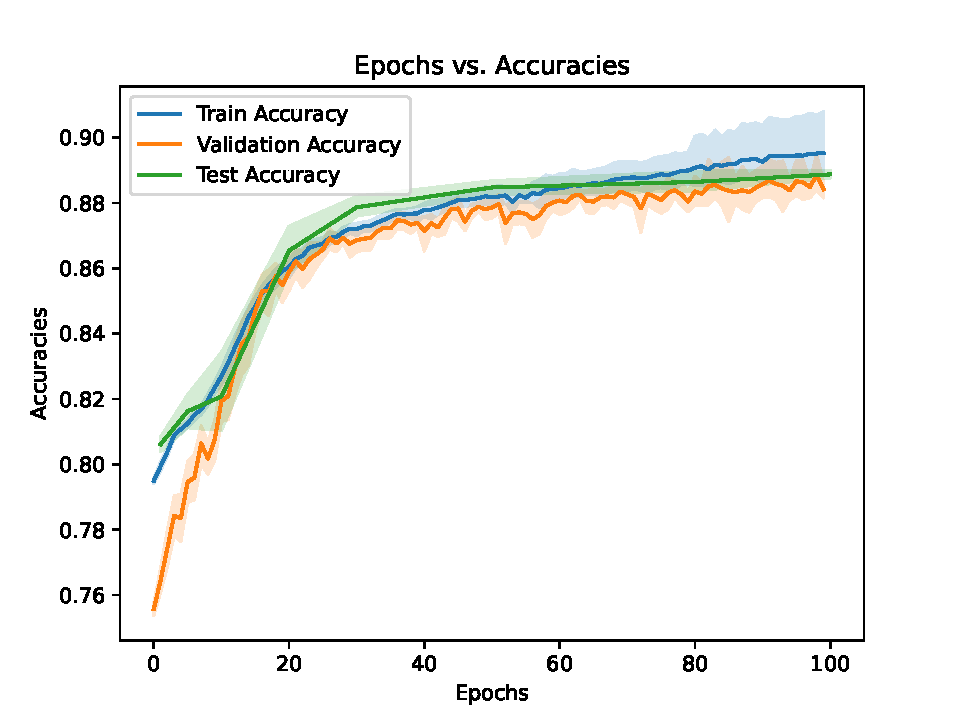
\includegraphics[width=1.0\columnwidth]{images/epoch_vs_accuracy.pdf}
\caption{Epoch vs accuracy.}
\label{fig:epochs-vs-accuracy-a}
\end{figure}


\begin{figure}[htb]
\centering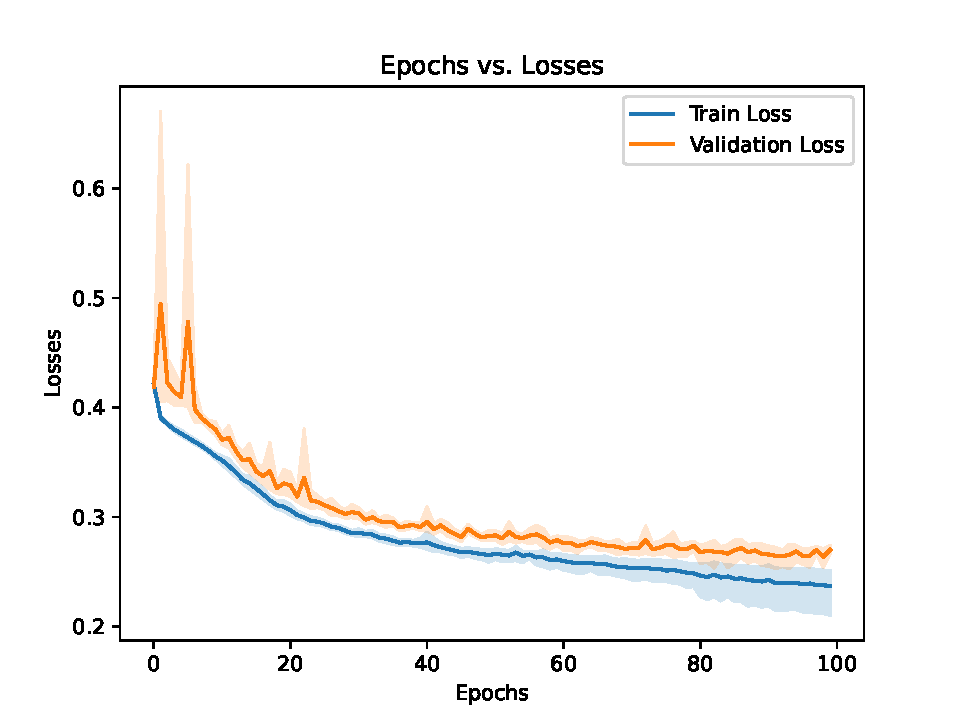
\includegraphics[width=1.0\columnwidth]{images/epoch_vs_loss.pdf}
\caption{Epoch vs loss.}
\label{fig:epochs-vs-accuracy-b}
\end{figure}


\begin{figure}[htb]
\centering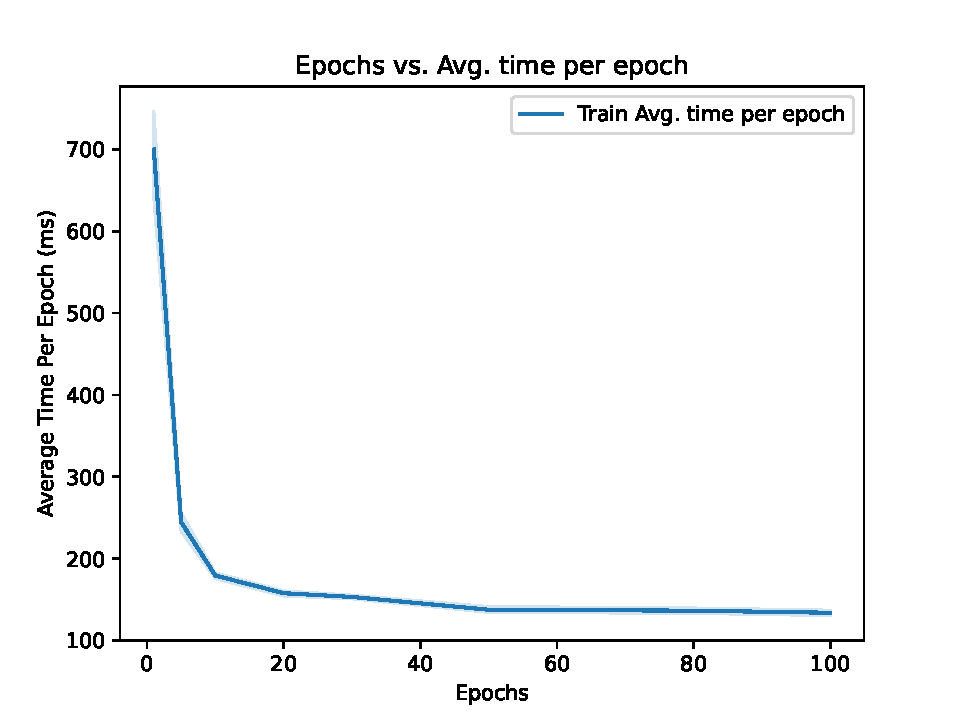
\includegraphics[width=1.0\columnwidth]{images/epoch_vs_train_time.pdf}
\caption{Epoch vs train time.}
\label{fig:epochs-vs-accuracy-c}
\end{figure}

\begin{figure}[htb]
\centering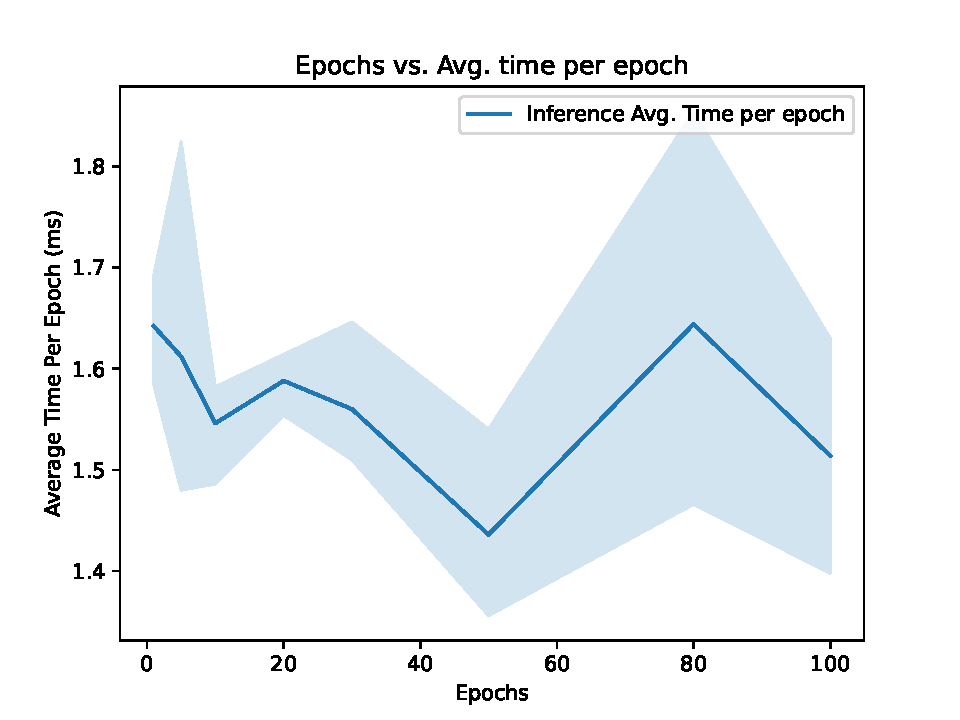
\includegraphics[width=1.0\columnwidth]{images/epoch_vs_test_time.pdf}
\caption{Epoch vs inference time.}
\label{fig:epochs-vs-accuracy-d}
\end{figure}

\begin{figure}[htb]
\centering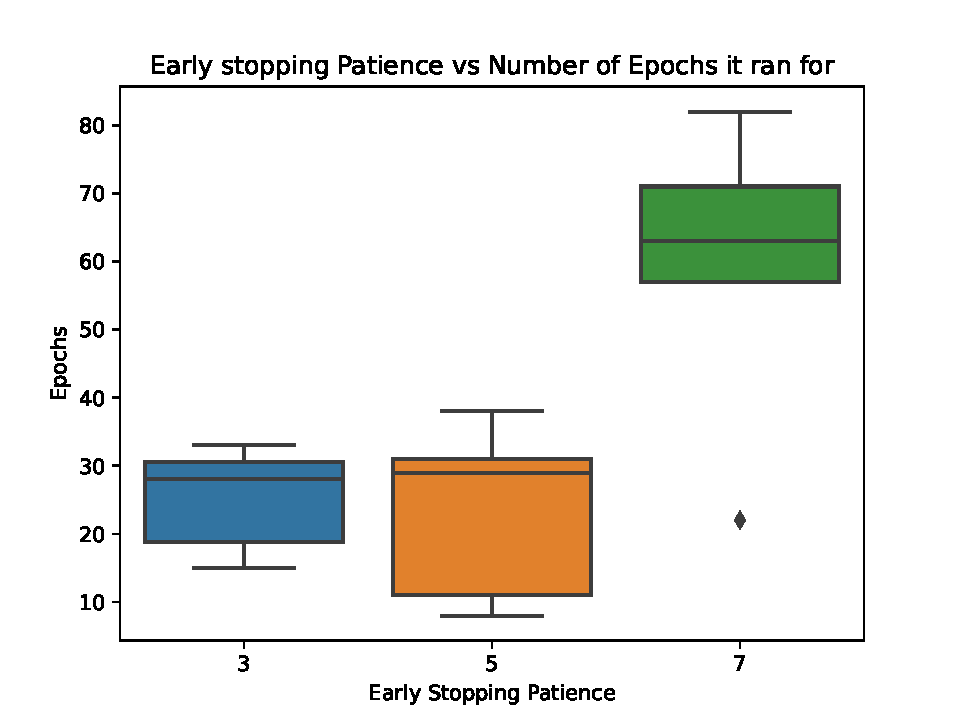
\includegraphics[width=1.0\columnwidth]{images/early_stopping.pdf}
\caption{Epoch vs inference time.}
\label{fig:early-stopping}
\end{figure}

\section{Results and Discussion}

\subsection{Benchmark Results}

\begin{itemize}
    \item Observations from the table
    \item Shortcomings of your study 
    \item Errors discovered by team
    \item Educational lessons
\end{itemize}




\subsection{Educational Lessons learned}


\TODO{what are the educational lessons learned from this example}

\TODO{What are the lessons learned from the particular approach used in this experience? E.g. how did splitup work. how did time management work ... what was the impact of the teammate leaving? things like this. Does the previous teammate need to be added to the acknowledgement? Maybe not as it then would reveal identity we could keep acknowledgment anonymous or not at all? Did the university program adequately prepare for HPC usage? Put some thoughts here ...}

\TODO{describe the organization of the team and if the team organization worked. Describe how work was performed.}

In addition to the team, the first author was always available for meetings and discussions. He engaged upon request in several hackathons to identify bugs and setup issues and scheduled several mandatory hackathons. These hackathons were attended by a single member of the NYU team. 
\TODO{please correct.}

\begin{comment}
The team elected to schedule meetings mostly n a two-week schedule. In the second semester, a meeting did not take place till the 4ths week of the semester.
\end{comment}


\section{Conclusion}
\label{sec:conclusion}

\TODO{missing}

\begin{acks}

Work was in part funded by the NSF CyberTraining: CIC: CyberTraining for Students and Technologies from Generation Z with the award numbers 1829704 and 2200409 and NIST 60NANB21D151T.  The work was also funded by the Department of Energy under the grant Award No. DE-SC0023452. The work was conducted at the Biocomplexity Institute and Initiative at the University of Virginia.

We like to thank Thomas Butler and J.P Fleisher for their contributions during the development of cloudmesh-sbatch and cloudmesh-cc.

\end{acks}

%%
%% The next two lines define the bibliography style to be used, and
%% the bibliography file.
\bibliographystyle{ACM-Reference-Format}
\bibliography{3-references}

%%
%% If your work has an appendix, this is the place to put it.
\appendix


\section{Appendix}

\section{Work conducted}

This section contains for each person what they contributed.

{\em GvL} functioned as a technical supervisor in this project and interfaced with the MLCommons Science Working group. He has spearheaded this project and ran several benchmarks on UVA's Rivanna machine and a desktop. He is the primary author of cloudmesh and cloudmesh-sbatch which is used in this project on Rivanna and the desktop to drastically simplify executions with permutations of hyperparameters. He is the author of cloudmesh StopWatch used in the code to measure the time.
{\em VC} is the primary developer at NYU that ported the application to Greene.  
{\em LM} helped in general with project management and contributed to the paper.
{\em RG} has contributed to this paper in multiple ways. He first improved the related research section and later contributed to reproducing the results on Greene while rerunning some experiments.
{\em GCF} is a Working group chair of the MLCommons Science Working Group. He initiated the project together with {\em SS}. {\em SS} is the academic supervisor of the participating students at NYU.

\subsection{Installation}

Put detailed installation instructions here

{\footnotesize
\begin{Verbatim}[numbers=left,xleftmargin=5mm]
cd ~
# commant
mkdir abc
git clone xyz
...
\end{Verbatim}
}

\subsection{Project Links}

% \TODO{create misc BibTeX entries and use them here and add after the href command the cite command}

The cloudmesh code for MLCommons is managed in the MLCommons Science repository \cite{github-laszewsk-mlcommons}
Within this directory, we have a number of subdirectories. One of them is \href{https://github.com/laszewsk/mlcommons/tree/main/benchmarks/cloudmask/experiments/rivanna}{benchmarks/experiment/greene}. For the NYU code. The other is \href{https://github.com/laszewsk/mlcommons/tree/main/benchmarks/cloudmask/experiments/rivanna}{benchmarks/experiment/rivanna} for the code to be run on UVA rivanna.

\begin{comment}
\begin{description}
\item[Zoom Meetings:] \href{https://virginia.zoom.us/j/5911267906}{link}
\item[Repo Gregor:] \item[Repo Vashita:] \href{https://github.com/VarshithaChennamsetti/mlcommons}{link}
\item[Issues:] 
\href{https://github.com/laszewsk/mlcommons/issues/50}{link}
\item[Notes:] \href{https://docs.google.com/document/d/1LUuVSeLYv-717TJxtyikihLmuyf6at50FNBn57Doo_4}{link}
\item[Overleaf:] \href{https://www.overleaf.com/project/634d9954592bab690b6d133d}{link}
\end{description}
\end{comment}

\section{Data Download Performance}

\TODO{This section has to be integrated into the benchmark section once completed}

The data used in the performance experiments is ?? GB big. 

While downloading it on the DGX station into the system-configured raid array we retrieved it in real time of 53m39.041s. Using ookolas speed test measured a download speed potential of 595.19 Mbit/s.


\begin{comment}
    
53m39.041s
user	7m46.329s
sys	5m25.439s
/raid/
Retrieving speedtest.net server list...
Hosted by Magna5 (Manassas, VA) 
[119.58 km]: 20.935 ms
Download: 595.19 Mbit/s
Upload: 41.80 Mbit/s

\end{comment}

Data from rivanna and greene missing

\TODO{Data from Greene missing}

\end{document}
\endinput
%%
%% End of file `sample-sigplan.tex'.
